\PassOptionsToPackage{unicode=true}{hyperref} % options for packages loaded elsewhere
\PassOptionsToPackage{hyphens}{url}
%
\documentclass[ignorenonframetext,]{beamer}
\usepackage{pgfpages}
\setbeamertemplate{caption}[numbered]
\setbeamertemplate{caption label separator}{: }
\setbeamercolor{caption name}{fg=normal text.fg}
\beamertemplatenavigationsymbolsempty
% Prevent slide breaks in the middle of a paragraph:
\widowpenalties 1 10000
\raggedbottom
\setbeamertemplate{part page}{
\centering
\begin{beamercolorbox}[sep=16pt,center]{part title}
  \usebeamerfont{part title}\insertpart\par
\end{beamercolorbox}
}
\setbeamertemplate{section page}{
\centering
\begin{beamercolorbox}[sep=12pt,center]{part title}
  \usebeamerfont{section title}\insertsection\par
\end{beamercolorbox}
}
\setbeamertemplate{subsection page}{
\centering
\begin{beamercolorbox}[sep=8pt,center]{part title}
  \usebeamerfont{subsection title}\insertsubsection\par
\end{beamercolorbox}
}
\AtBeginPart{
  \frame{\partpage}
}
\AtBeginSection{
  \ifbibliography
  \else
    \frame{\sectionpage}
  \fi
}
\AtBeginSubsection{
  \frame{\subsectionpage}
}
\usepackage{lmodern}
\usepackage{amssymb,amsmath}
\usepackage{ifxetex,ifluatex}
\usepackage{fixltx2e} % provides \textsubscript
\ifnum 0\ifxetex 1\fi\ifluatex 1\fi=0 % if pdftex
  \usepackage[T1]{fontenc}
  \usepackage[utf8]{inputenc}
  \usepackage{textcomp} % provides euro and other symbols
\else % if luatex or xelatex
  \usepackage{unicode-math}
  \defaultfontfeatures{Ligatures=TeX,Scale=MatchLowercase}
\fi
% use upquote if available, for straight quotes in verbatim environments
\IfFileExists{upquote.sty}{\usepackage{upquote}}{}
% use microtype if available
\IfFileExists{microtype.sty}{%
\usepackage[]{microtype}
\UseMicrotypeSet[protrusion]{basicmath} % disable protrusion for tt fonts
}{}
\IfFileExists{parskip.sty}{%
\usepackage{parskip}
}{% else
\setlength{\parindent}{0pt}
\setlength{\parskip}{6pt plus 2pt minus 1pt}
}
\usepackage{hyperref}
\hypersetup{
            pdftitle={Marketing Science with R},
            pdfauthor={TokyoR \#78 Kien Knot(きぬいと; @0\_u0)},
            pdfborder={0 0 0},
            breaklinks=true}
\urlstyle{same}  % don't use monospace font for urls
\newif\ifbibliography
\usepackage{graphicx,grffile}
\makeatletter
\def\maxwidth{\ifdim\Gin@nat@width>\linewidth\linewidth\else\Gin@nat@width\fi}
\def\maxheight{\ifdim\Gin@nat@height>\textheight\textheight\else\Gin@nat@height\fi}
\makeatother
% Scale images if necessary, so that they will not overflow the page
% margins by default, and it is still possible to overwrite the defaults
% using explicit options in \includegraphics[width, height, ...]{}
\setkeys{Gin}{width=\maxwidth,height=\maxheight,keepaspectratio}
\setlength{\emergencystretch}{3em}  % prevent overfull lines
\providecommand{\tightlist}{%
  \setlength{\itemsep}{0pt}\setlength{\parskip}{0pt}}
\setcounter{secnumdepth}{0}

% set default figure placement to htbp
\makeatletter
\def\fps@figure{htbp}
\makeatother


\title{Marketing Science with R}
\author{TokyoR \#78 Kien Knot(きぬいと; @0\_u0)}
\date{2019/5/25}

\begin{document}
\frame{\titlepage}

\section{はじめに}

\begin{frame}{自己紹介}

\begin{itemize}
\tightlist
\item
  労働者階級2年目

  \begin{itemize}
  \tightlist
  \item
    マーケティング系調査屋さんのアナリスト

    \begin{itemize}
    \tightlist
    \item
      兼アナリスト候補のヘッドハンター
    \item
      兼部署内作業環境改善係
    \item
      兼広報担当
    \end{itemize}
  \end{itemize}
\item
  最近の出来事

  \begin{itemize}
  \tightlist
  \item
    転職しないことにした

    \begin{itemize}
    \tightlist
    \item
      キャリアなんもわからん問題でバズってしまった
    \item
      なお今もなんもわからん模様
    \end{itemize}
  \item
    OSをUbuntuに変えたらMSOffice使えないじゃない

    \begin{itemize}
    \tightlist
    \item
      Rmdで資料を作る環境を「無理やり」作り上げた
    \end{itemize}
  \end{itemize}
\end{itemize}

\end{frame}

\begin{frame}{宣伝}

\begin{itemize}
\tightlist
\item
  Statistician-jaのDiscordをつくりました

  \begin{itemize}
  \tightlist
  \item
    「数理統計学」をやっていくサーバ

    \begin{itemize}
    \tightlist
    \item
      「10人くらいかなあ」→300人超えてきた
    \end{itemize}
  \end{itemize}
\end{itemize}

\end{frame}

\begin{frame}{宣伝}
\protect\hypertarget{-1}{}

\includegraphics{./Presentation_files/Thinker.jpg}

\end{frame}

\begin{frame}[fragile]{宣伝}
\protect\hypertarget{-2}{}

\begin{itemize}
\tightlist
\item
  PythonとかRとかではなく「数理統計」のお勉強をやろう

  \begin{itemize}
  \tightlist
  \item
    \texttt{lm(y\textasciitilde{}.,\ data\ =\ dat)}の裏のロジックをつかもう
  \end{itemize}
\item
  目標は統計検定1級に合格することなど
\item
  \url{https://discord.gg/Nq75Smp}にアクセスしてみんなも強くなろう!

  \begin{itemize}
  \tightlist
  \item
    Meetupとかも構想中です。
  \end{itemize}
\end{itemize}

\end{frame}

\begin{frame}{今日のお話}

\begin{itemize}
\tightlist
\item
  「Rって非Teck系企業でどう使われているんですか?」なお話

  \begin{itemize}
  \tightlist
  \item
    R: エンジニアじゃない人も割と使ってる
  \item
    故に「バージョン管理」とかよく分かってないことも多く\ldots{}\ldots{}
  \end{itemize}
\item
  エンジニアじゃないのでこの辺のソース管理とか教えてほしいです

  \begin{itemize}
  \tightlist
  \item
    最近社内で\href{https://speakerdeck.com/s_uryu/rstudio-for-team}{Uribo先生の資料}を紹介しました
  \end{itemize}
\end{itemize}

\end{frame}

\begin{frame}{今日のお話}
\protect\hypertarget{-1}{}

\begin{itemize}
\tightlist
\item
  マーケティング・サイエンスの分野で使われるRの話

  \begin{itemize}
  \tightlist
  \item
    ヤバイ強いきかいがくしゅーとかでてこない

    \begin{itemize}
    \tightlist
    \item
      この話は次回やります
    \end{itemize}
  \end{itemize}
\item
  R要素は?

  \begin{itemize}
  \tightlist
  \item
    これがRmarkdownでできている
  \item
    それで十分じゃないか\ldots{}\ldots{}?
  \item
    ioslideの無骨さいい\ldots{}\ldots{}
  \end{itemize}
\end{itemize}

\end{frame}

\section{「マーケティング」って何?}

\begin{frame}[fragile]{実際に聞いてみたい}

\begin{itemize}
\tightlist
\item
  Q.「マーケティングってなんだと思いますか?」
\end{itemize}

\begin{verbatim}
## Warning in axis(if (horiz) 2 else 1, at = at.l, labels = names.arg, lty =
## axis.lty, : 'mbcsToSbcs' 中の '1.よくわからない' で変換に失敗: <e3> をドッ
## トで置き換えました
\end{verbatim}

\begin{verbatim}
## Warning in axis(if (horiz) 2 else 1, at = at.l, labels = names.arg, lty =
## axis.lty, : 'mbcsToSbcs' 中の '1.よくわからない' で変換に失敗: <82> をドッ
## トで置き換えました
\end{verbatim}

\begin{verbatim}
## Warning in axis(if (horiz) 2 else 1, at = at.l, labels = names.arg, lty =
## axis.lty, : 'mbcsToSbcs' 中の '1.よくわからない' で変換に失敗: <88> をドッ
## トで置き換えました
\end{verbatim}

\begin{verbatim}
## Warning in axis(if (horiz) 2 else 1, at = at.l, labels = names.arg, lty =
## axis.lty, : 'mbcsToSbcs' 中の '1.よくわからない' で変換に失敗: <e3> をドッ
## トで置き換えました
\end{verbatim}

\begin{verbatim}
## Warning in axis(if (horiz) 2 else 1, at = at.l, labels = names.arg, lty =
## axis.lty, : 'mbcsToSbcs' 中の '1.よくわからない' で変換に失敗: <81> をドッ
## トで置き換えました
\end{verbatim}

\begin{verbatim}
## Warning in axis(if (horiz) 2 else 1, at = at.l, labels = names.arg, lty =
## axis.lty, : 'mbcsToSbcs' 中の '1.よくわからない' で変換に失敗: <8f> をドッ
## トで置き換えました
\end{verbatim}

\begin{verbatim}
## Warning in axis(if (horiz) 2 else 1, at = at.l, labels = names.arg, lty =
## axis.lty, : 'mbcsToSbcs' 中の '1.よくわからない' で変換に失敗: <e3> をドッ
## トで置き換えました
\end{verbatim}

\begin{verbatim}
## Warning in axis(if (horiz) 2 else 1, at = at.l, labels = names.arg, lty =
## axis.lty, : 'mbcsToSbcs' 中の '1.よくわからない' で変換に失敗: <82> をドッ
## トで置き換えました
\end{verbatim}

\begin{verbatim}
## Warning in axis(if (horiz) 2 else 1, at = at.l, labels = names.arg, lty =
## axis.lty, : 'mbcsToSbcs' 中の '1.よくわからない' で変換に失敗: <8f> をドッ
## トで置き換えました
\end{verbatim}

\begin{verbatim}
## Warning in axis(if (horiz) 2 else 1, at = at.l, labels = names.arg, lty =
## axis.lty, : 'mbcsToSbcs' 中の '1.よくわからない' で変換に失敗: <e3> をドッ
## トで置き換えました
\end{verbatim}

\begin{verbatim}
## Warning in axis(if (horiz) 2 else 1, at = at.l, labels = names.arg, lty =
## axis.lty, : 'mbcsToSbcs' 中の '1.よくわからない' で変換に失敗: <81> をドッ
## トで置き換えました
\end{verbatim}

\begin{verbatim}
## Warning in axis(if (horiz) 2 else 1, at = at.l, labels = names.arg, lty =
## axis.lty, : 'mbcsToSbcs' 中の '1.よくわからない' で変換に失敗: <8b> をドッ
## トで置き換えました
\end{verbatim}

\begin{verbatim}
## Warning in axis(if (horiz) 2 else 1, at = at.l, labels = names.arg, lty =
## axis.lty, : 'mbcsToSbcs' 中の '1.よくわからない' で変換に失敗: <e3> をドッ
## トで置き換えました
\end{verbatim}

\begin{verbatim}
## Warning in axis(if (horiz) 2 else 1, at = at.l, labels = names.arg, lty =
## axis.lty, : 'mbcsToSbcs' 中の '1.よくわからない' で変換に失敗: <82> をドッ
## トで置き換えました
\end{verbatim}

\begin{verbatim}
## Warning in axis(if (horiz) 2 else 1, at = at.l, labels = names.arg, lty =
## axis.lty, : 'mbcsToSbcs' 中の '1.よくわからない' で変換に失敗: <89> をドッ
## トで置き換えました
\end{verbatim}

\begin{verbatim}
## Warning in axis(if (horiz) 2 else 1, at = at.l, labels = names.arg, lty =
## axis.lty, : 'mbcsToSbcs' 中の '1.よくわからない' で変換に失敗: <e3> をドッ
## トで置き換えました
\end{verbatim}

\begin{verbatim}
## Warning in axis(if (horiz) 2 else 1, at = at.l, labels = names.arg, lty =
## axis.lty, : 'mbcsToSbcs' 中の '1.よくわからない' で変換に失敗: <81> をドッ
## トで置き換えました
\end{verbatim}

\begin{verbatim}
## Warning in axis(if (horiz) 2 else 1, at = at.l, labels = names.arg, lty =
## axis.lty, : 'mbcsToSbcs' 中の '1.よくわからない' で変換に失敗: <aa> をドッ
## トで置き換えました
\end{verbatim}

\begin{verbatim}
## Warning in axis(if (horiz) 2 else 1, at = at.l, labels = names.arg, lty =
## axis.lty, : 'mbcsToSbcs' 中の '1.よくわからない' で変換に失敗: <e3> をドッ
## トで置き換えました
\end{verbatim}

\begin{verbatim}
## Warning in axis(if (horiz) 2 else 1, at = at.l, labels = names.arg, lty =
## axis.lty, : 'mbcsToSbcs' 中の '1.よくわからない' で変換に失敗: <81> をドッ
## トで置き換えました
\end{verbatim}

\begin{verbatim}
## Warning in axis(if (horiz) 2 else 1, at = at.l, labels = names.arg, lty =
## axis.lty, : 'mbcsToSbcs' 中の '1.よくわからない' で変換に失敗: <84> をドッ
## トで置き換えました
\end{verbatim}

\begin{verbatim}
## Warning in axis(if (horiz) 2 else 1, at = at.l, labels = names.arg, lty =
## axis.lty, : 'mbcsToSbcs' 中の '1.よくわからない' で変換に失敗: <e3> をドッ
## トで置き換えました
\end{verbatim}

\begin{verbatim}
## Warning in axis(if (horiz) 2 else 1, at = at.l, labels = names.arg, lty =
## axis.lty, : 'mbcsToSbcs' 中の '1.よくわからない' で変換に失敗: <82> をドッ
## トで置き換えました
\end{verbatim}

\begin{verbatim}
## Warning in axis(if (horiz) 2 else 1, at = at.l, labels = names.arg, lty =
## axis.lty, : 'mbcsToSbcs' 中の '1.よくわからない' で変換に失敗: <88> をドッ
## トで置き換えました
\end{verbatim}

\begin{verbatim}
## Warning in axis(if (horiz) 2 else 1, at = at.l, labels = names.arg, lty =
## axis.lty, : 'mbcsToSbcs' 中の '1.よくわからない' で変換に失敗: <e3> をドッ
## トで置き換えました
\end{verbatim}

\begin{verbatim}
## Warning in axis(if (horiz) 2 else 1, at = at.l, labels = names.arg, lty =
## axis.lty, : 'mbcsToSbcs' 中の '1.よくわからない' で変換に失敗: <81> をドッ
## トで置き換えました
\end{verbatim}

\begin{verbatim}
## Warning in axis(if (horiz) 2 else 1, at = at.l, labels = names.arg, lty =
## axis.lty, : 'mbcsToSbcs' 中の '1.よくわからない' で変換に失敗: <8f> をドッ
## トで置き換えました
\end{verbatim}

\begin{verbatim}
## Warning in axis(if (horiz) 2 else 1, at = at.l, labels = names.arg, lty =
## axis.lty, : 'mbcsToSbcs' 中の '1.よくわからない' で変換に失敗: <e3> をドッ
## トで置き換えました
\end{verbatim}

\begin{verbatim}
## Warning in axis(if (horiz) 2 else 1, at = at.l, labels = names.arg, lty =
## axis.lty, : 'mbcsToSbcs' 中の '1.よくわからない' で変換に失敗: <82> をドッ
## トで置き換えました
\end{verbatim}

\begin{verbatim}
## Warning in axis(if (horiz) 2 else 1, at = at.l, labels = names.arg, lty =
## axis.lty, : 'mbcsToSbcs' 中の '1.よくわからない' で変換に失敗: <8f> をドッ
## トで置き換えました
\end{verbatim}

\begin{verbatim}
## Warning in axis(if (horiz) 2 else 1, at = at.l, labels = names.arg, lty =
## axis.lty, : 'mbcsToSbcs' 中の '1.よくわからない' で変換に失敗: <e3> をドッ
## トで置き換えました
\end{verbatim}

\begin{verbatim}
## Warning in axis(if (horiz) 2 else 1, at = at.l, labels = names.arg, lty =
## axis.lty, : 'mbcsToSbcs' 中の '1.よくわからない' で変換に失敗: <81> をドッ
## トで置き換えました
\end{verbatim}

\begin{verbatim}
## Warning in axis(if (horiz) 2 else 1, at = at.l, labels = names.arg, lty =
## axis.lty, : 'mbcsToSbcs' 中の '1.よくわからない' で変換に失敗: <8b> をドッ
## トで置き換えました
\end{verbatim}

\begin{verbatim}
## Warning in axis(if (horiz) 2 else 1, at = at.l, labels = names.arg, lty =
## axis.lty, : 'mbcsToSbcs' 中の '1.よくわからない' で変換に失敗: <e3> をドッ
## トで置き換えました
\end{verbatim}

\begin{verbatim}
## Warning in axis(if (horiz) 2 else 1, at = at.l, labels = names.arg, lty =
## axis.lty, : 'mbcsToSbcs' 中の '1.よくわからない' で変換に失敗: <82> をドッ
## トで置き換えました
\end{verbatim}

\begin{verbatim}
## Warning in axis(if (horiz) 2 else 1, at = at.l, labels = names.arg, lty =
## axis.lty, : 'mbcsToSbcs' 中の '1.よくわからない' で変換に失敗: <89> をドッ
## トで置き換えました
\end{verbatim}

\begin{verbatim}
## Warning in axis(if (horiz) 2 else 1, at = at.l, labels = names.arg, lty =
## axis.lty, : 'mbcsToSbcs' 中の '1.よくわからない' で変換に失敗: <e3> をドッ
## トで置き換えました
\end{verbatim}

\begin{verbatim}
## Warning in axis(if (horiz) 2 else 1, at = at.l, labels = names.arg, lty =
## axis.lty, : 'mbcsToSbcs' 中の '1.よくわからない' で変換に失敗: <81> をドッ
## トで置き換えました
\end{verbatim}

\begin{verbatim}
## Warning in axis(if (horiz) 2 else 1, at = at.l, labels = names.arg, lty =
## axis.lty, : 'mbcsToSbcs' 中の '1.よくわからない' で変換に失敗: <aa> をドッ
## トで置き換えました
\end{verbatim}

\begin{verbatim}
## Warning in axis(if (horiz) 2 else 1, at = at.l, labels = names.arg, lty =
## axis.lty, : 'mbcsToSbcs' 中の '1.よくわからない' で変換に失敗: <e3> をドッ
## トで置き換えました
\end{verbatim}

\begin{verbatim}
## Warning in axis(if (horiz) 2 else 1, at = at.l, labels = names.arg, lty =
## axis.lty, : 'mbcsToSbcs' 中の '1.よくわからない' で変換に失敗: <81> をドッ
## トで置き換えました
\end{verbatim}

\begin{verbatim}
## Warning in axis(if (horiz) 2 else 1, at = at.l, labels = names.arg, lty =
## axis.lty, : 'mbcsToSbcs' 中の '1.よくわからない' で変換に失敗: <84> をドッ
## トで置き換えました
\end{verbatim}

\begin{verbatim}
## Warning in axis(if (horiz) 2 else 1, at = at.l, labels = names.arg, lty =
## axis.lty, : 'mbcsToSbcs' 中の '2.意識高い' で変換に失敗: <e6> をドットで置
## き換えました
\end{verbatim}

\begin{verbatim}
## Warning in axis(if (horiz) 2 else 1, at = at.l, labels = names.arg, lty =
## axis.lty, : 'mbcsToSbcs' 中の '2.意識高い' で変換に失敗: <84> をドットで置
## き換えました
\end{verbatim}

\begin{verbatim}
## Warning in axis(if (horiz) 2 else 1, at = at.l, labels = names.arg, lty =
## axis.lty, : 'mbcsToSbcs' 中の '2.意識高い' で変換に失敗: <8f> をドットで置
## き換えました
\end{verbatim}

\begin{verbatim}
## Warning in axis(if (horiz) 2 else 1, at = at.l, labels = names.arg, lty =
## axis.lty, : 'mbcsToSbcs' 中の '2.意識高い' で変換に失敗: <e8> をドットで置
## き換えました
\end{verbatim}

\begin{verbatim}
## Warning in axis(if (horiz) 2 else 1, at = at.l, labels = names.arg, lty =
## axis.lty, : 'mbcsToSbcs' 中の '2.意識高い' で変換に失敗: <ad> をドットで置
## き換えました
\end{verbatim}

\begin{verbatim}
## Warning in axis(if (horiz) 2 else 1, at = at.l, labels = names.arg, lty =
## axis.lty, : 'mbcsToSbcs' 中の '2.意識高い' で変換に失敗: <98> をドットで置
## き換えました
\end{verbatim}

\begin{verbatim}
## Warning in axis(if (horiz) 2 else 1, at = at.l, labels = names.arg, lty =
## axis.lty, : 'mbcsToSbcs' 中の '2.意識高い' で変換に失敗: <e9> をドットで置
## き換えました
\end{verbatim}

\begin{verbatim}
## Warning in axis(if (horiz) 2 else 1, at = at.l, labels = names.arg, lty =
## axis.lty, : 'mbcsToSbcs' 中の '2.意識高い' で変換に失敗: <ab> をドットで置
## き換えました
\end{verbatim}

\begin{verbatim}
## Warning in axis(if (horiz) 2 else 1, at = at.l, labels = names.arg, lty =
## axis.lty, : 'mbcsToSbcs' 中の '2.意識高い' で変換に失敗: <98> をドットで置
## き換えました
\end{verbatim}

\begin{verbatim}
## Warning in axis(if (horiz) 2 else 1, at = at.l, labels = names.arg, lty =
## axis.lty, : 'mbcsToSbcs' 中の '2.意識高い' で変換に失敗: <e3> をドットで置
## き換えました
\end{verbatim}

\begin{verbatim}
## Warning in axis(if (horiz) 2 else 1, at = at.l, labels = names.arg, lty =
## axis.lty, : 'mbcsToSbcs' 中の '2.意識高い' で変換に失敗: <81> をドットで置
## き換えました
\end{verbatim}

\begin{verbatim}
## Warning in axis(if (horiz) 2 else 1, at = at.l, labels = names.arg, lty =
## axis.lty, : 'mbcsToSbcs' 中の '2.意識高い' で変換に失敗: <84> をドットで置
## き換えました
\end{verbatim}

\begin{verbatim}
## Warning in axis(if (horiz) 2 else 1, at = at.l, labels = names.arg, lty =
## axis.lty, : 'mbcsToSbcs' 中の '2.意識高い' で変換に失敗: <e6> をドットで置
## き換えました
\end{verbatim}

\begin{verbatim}
## Warning in axis(if (horiz) 2 else 1, at = at.l, labels = names.arg, lty =
## axis.lty, : 'mbcsToSbcs' 中の '2.意識高い' で変換に失敗: <84> をドットで置
## き換えました
\end{verbatim}

\begin{verbatim}
## Warning in axis(if (horiz) 2 else 1, at = at.l, labels = names.arg, lty =
## axis.lty, : 'mbcsToSbcs' 中の '2.意識高い' で変換に失敗: <8f> をドットで置
## き換えました
\end{verbatim}

\begin{verbatim}
## Warning in axis(if (horiz) 2 else 1, at = at.l, labels = names.arg, lty =
## axis.lty, : 'mbcsToSbcs' 中の '2.意識高い' で変換に失敗: <e8> をドットで置
## き換えました
\end{verbatim}

\begin{verbatim}
## Warning in axis(if (horiz) 2 else 1, at = at.l, labels = names.arg, lty =
## axis.lty, : 'mbcsToSbcs' 中の '2.意識高い' で変換に失敗: <ad> をドットで置
## き換えました
\end{verbatim}

\begin{verbatim}
## Warning in axis(if (horiz) 2 else 1, at = at.l, labels = names.arg, lty =
## axis.lty, : 'mbcsToSbcs' 中の '2.意識高い' で変換に失敗: <98> をドットで置
## き換えました
\end{verbatim}

\begin{verbatim}
## Warning in axis(if (horiz) 2 else 1, at = at.l, labels = names.arg, lty =
## axis.lty, : 'mbcsToSbcs' 中の '2.意識高い' で変換に失敗: <e9> をドットで置
## き換えました
\end{verbatim}

\begin{verbatim}
## Warning in axis(if (horiz) 2 else 1, at = at.l, labels = names.arg, lty =
## axis.lty, : 'mbcsToSbcs' 中の '2.意識高い' で変換に失敗: <ab> をドットで置
## き換えました
\end{verbatim}

\begin{verbatim}
## Warning in axis(if (horiz) 2 else 1, at = at.l, labels = names.arg, lty =
## axis.lty, : 'mbcsToSbcs' 中の '2.意識高い' で変換に失敗: <98> をドットで置
## き換えました
\end{verbatim}

\begin{verbatim}
## Warning in axis(if (horiz) 2 else 1, at = at.l, labels = names.arg, lty =
## axis.lty, : 'mbcsToSbcs' 中の '2.意識高い' で変換に失敗: <e3> をドットで置
## き換えました
\end{verbatim}

\begin{verbatim}
## Warning in axis(if (horiz) 2 else 1, at = at.l, labels = names.arg, lty =
## axis.lty, : 'mbcsToSbcs' 中の '2.意識高い' で変換に失敗: <81> をドットで置
## き換えました
\end{verbatim}

\begin{verbatim}
## Warning in axis(if (horiz) 2 else 1, at = at.l, labels = names.arg, lty =
## axis.lty, : 'mbcsToSbcs' 中の '2.意識高い' で変換に失敗: <84> をドットで置
## き換えました
\end{verbatim}

\begin{verbatim}
## Warning in axis(if (horiz) 2 else 1, at = at.l, labels = names.arg, lty =
## axis.lty, : 'mbcsToSbcs' 中の '3.2020年代最もセクシーな仕事' で変換に失敗:
## <e5> をドットで置き換えました
\end{verbatim}

\begin{verbatim}
## Warning in axis(if (horiz) 2 else 1, at = at.l, labels = names.arg, lty =
## axis.lty, : 'mbcsToSbcs' 中の '3.2020年代最もセクシーな仕事' で変換に失敗:
## <b9> をドットで置き換えました
\end{verbatim}

\begin{verbatim}
## Warning in axis(if (horiz) 2 else 1, at = at.l, labels = names.arg, lty =
## axis.lty, : 'mbcsToSbcs' 中の '3.2020年代最もセクシーな仕事' で変換に失敗:
## <b4> をドットで置き換えました
\end{verbatim}

\begin{verbatim}
## Warning in axis(if (horiz) 2 else 1, at = at.l, labels = names.arg, lty =
## axis.lty, : 'mbcsToSbcs' 中の '3.2020年代最もセクシーな仕事' で変換に失敗:
## <e4> をドットで置き換えました
\end{verbatim}

\begin{verbatim}
## Warning in axis(if (horiz) 2 else 1, at = at.l, labels = names.arg, lty =
## axis.lty, : 'mbcsToSbcs' 中の '3.2020年代最もセクシーな仕事' で変換に失敗:
## <bb> をドットで置き換えました
\end{verbatim}

\begin{verbatim}
## Warning in axis(if (horiz) 2 else 1, at = at.l, labels = names.arg, lty =
## axis.lty, : 'mbcsToSbcs' 中の '3.2020年代最もセクシーな仕事' で変換に失敗:
## <a3> をドットで置き換えました
\end{verbatim}

\begin{verbatim}
## Warning in axis(if (horiz) 2 else 1, at = at.l, labels = names.arg, lty =
## axis.lty, : 'mbcsToSbcs' 中の '3.2020年代最もセクシーな仕事' で変換に失敗:
## <e6> をドットで置き換えました
\end{verbatim}

\begin{verbatim}
## Warning in axis(if (horiz) 2 else 1, at = at.l, labels = names.arg, lty =
## axis.lty, : 'mbcsToSbcs' 中の '3.2020年代最もセクシーな仕事' で変換に失敗:
## <9c> をドットで置き換えました
\end{verbatim}

\begin{verbatim}
## Warning in axis(if (horiz) 2 else 1, at = at.l, labels = names.arg, lty =
## axis.lty, : 'mbcsToSbcs' 中の '3.2020年代最もセクシーな仕事' で変換に失敗:
## <80> をドットで置き換えました
\end{verbatim}

\begin{verbatim}
## Warning in axis(if (horiz) 2 else 1, at = at.l, labels = names.arg, lty =
## axis.lty, : 'mbcsToSbcs' 中の '3.2020年代最もセクシーな仕事' で変換に失敗:
## <e3> をドットで置き換えました
\end{verbatim}

\begin{verbatim}
## Warning in axis(if (horiz) 2 else 1, at = at.l, labels = names.arg, lty =
## axis.lty, : 'mbcsToSbcs' 中の '3.2020年代最もセクシーな仕事' で変換に失敗:
## <82> をドットで置き換えました

## Warning in axis(if (horiz) 2 else 1, at = at.l, labels = names.arg, lty =
## axis.lty, : 'mbcsToSbcs' 中の '3.2020年代最もセクシーな仕事' で変換に失敗:
## <82> をドットで置き換えました
\end{verbatim}

\begin{verbatim}
## Warning in axis(if (horiz) 2 else 1, at = at.l, labels = names.arg, lty =
## axis.lty, : 'mbcsToSbcs' 中の '3.2020年代最もセクシーな仕事' で変換に失敗:
## <e3> をドットで置き換えました
\end{verbatim}

\begin{verbatim}
## Warning in axis(if (horiz) 2 else 1, at = at.l, labels = names.arg, lty =
## axis.lty, : 'mbcsToSbcs' 中の '3.2020年代最もセクシーな仕事' で変換に失敗:
## <82> をドットで置き換えました
\end{verbatim}

\begin{verbatim}
## Warning in axis(if (horiz) 2 else 1, at = at.l, labels = names.arg, lty =
## axis.lty, : 'mbcsToSbcs' 中の '3.2020年代最もセクシーな仕事' で変換に失敗:
## <bb> をドットで置き換えました
\end{verbatim}

\begin{verbatim}
## Warning in axis(if (horiz) 2 else 1, at = at.l, labels = names.arg, lty =
## axis.lty, : 'mbcsToSbcs' 中の '3.2020年代最もセクシーな仕事' で変換に失敗:
## <e3> をドットで置き換えました
\end{verbatim}

\begin{verbatim}
## Warning in axis(if (horiz) 2 else 1, at = at.l, labels = names.arg, lty =
## axis.lty, : 'mbcsToSbcs' 中の '3.2020年代最もセクシーな仕事' で変換に失敗:
## <82> をドットで置き換えました
\end{verbatim}

\begin{verbatim}
## Warning in axis(if (horiz) 2 else 1, at = at.l, labels = names.arg, lty =
## axis.lty, : 'mbcsToSbcs' 中の '3.2020年代最もセクシーな仕事' で変換に失敗:
## <af> をドットで置き換えました
\end{verbatim}

\begin{verbatim}
## Warning in axis(if (horiz) 2 else 1, at = at.l, labels = names.arg, lty =
## axis.lty, : 'mbcsToSbcs' 中の '3.2020年代最もセクシーな仕事' で変換に失敗:
## <e3> をドットで置き換えました
\end{verbatim}

\begin{verbatim}
## Warning in axis(if (horiz) 2 else 1, at = at.l, labels = names.arg, lty =
## axis.lty, : 'mbcsToSbcs' 中の '3.2020年代最もセクシーな仕事' で変換に失敗:
## <82> をドットで置き換えました
\end{verbatim}

\begin{verbatim}
## Warning in axis(if (horiz) 2 else 1, at = at.l, labels = names.arg, lty =
## axis.lty, : 'mbcsToSbcs' 中の '3.2020年代最もセクシーな仕事' で変換に失敗:
## <b7> をドットで置き換えました
\end{verbatim}

\begin{verbatim}
## Warning in axis(if (horiz) 2 else 1, at = at.l, labels = names.arg, lty =
## axis.lty, : 'mbcsToSbcs' 中の '3.2020年代最もセクシーな仕事' で変換に失敗:
## <e3> をドットで置き換えました
\end{verbatim}

\begin{verbatim}
## Warning in axis(if (horiz) 2 else 1, at = at.l, labels = names.arg, lty =
## axis.lty, : 'mbcsToSbcs' 中の '3.2020年代最もセクシーな仕事' で変換に失敗:
## <83> をドットで置き換えました
\end{verbatim}

\begin{verbatim}
## Warning in axis(if (horiz) 2 else 1, at = at.l, labels = names.arg, lty =
## axis.lty, : 'mbcsToSbcs' 中の '3.2020年代最もセクシーな仕事' で変換に失敗:
## <bc> をドットで置き換えました
\end{verbatim}

\begin{verbatim}
## Warning in axis(if (horiz) 2 else 1, at = at.l, labels = names.arg, lty =
## axis.lty, : 'mbcsToSbcs' 中の '3.2020年代最もセクシーな仕事' で変換に失敗:
## <e3> をドットで置き換えました
\end{verbatim}

\begin{verbatim}
## Warning in axis(if (horiz) 2 else 1, at = at.l, labels = names.arg, lty =
## axis.lty, : 'mbcsToSbcs' 中の '3.2020年代最もセクシーな仕事' で変換に失敗:
## <81> をドットで置き換えました
\end{verbatim}

\begin{verbatim}
## Warning in axis(if (horiz) 2 else 1, at = at.l, labels = names.arg, lty =
## axis.lty, : 'mbcsToSbcs' 中の '3.2020年代最もセクシーな仕事' で変換に失敗:
## <aa> をドットで置き換えました
\end{verbatim}

\begin{verbatim}
## Warning in axis(if (horiz) 2 else 1, at = at.l, labels = names.arg, lty =
## axis.lty, : 'mbcsToSbcs' 中の '3.2020年代最もセクシーな仕事' で変換に失敗:
## <e4> をドットで置き換えました
\end{verbatim}

\begin{verbatim}
## Warning in axis(if (horiz) 2 else 1, at = at.l, labels = names.arg, lty =
## axis.lty, : 'mbcsToSbcs' 中の '3.2020年代最もセクシーな仕事' で変換に失敗:
## <bb> をドットで置き換えました
\end{verbatim}

\begin{verbatim}
## Warning in axis(if (horiz) 2 else 1, at = at.l, labels = names.arg, lty =
## axis.lty, : 'mbcsToSbcs' 中の '3.2020年代最もセクシーな仕事' で変換に失敗:
## <95> をドットで置き換えました
\end{verbatim}

\begin{verbatim}
## Warning in axis(if (horiz) 2 else 1, at = at.l, labels = names.arg, lty =
## axis.lty, : 'mbcsToSbcs' 中の '3.2020年代最もセクシーな仕事' で変換に失敗:
## <e4> をドットで置き換えました
\end{verbatim}

\begin{verbatim}
## Warning in axis(if (horiz) 2 else 1, at = at.l, labels = names.arg, lty =
## axis.lty, : 'mbcsToSbcs' 中の '3.2020年代最もセクシーな仕事' で変換に失敗:
## <ba> をドットで置き換えました
\end{verbatim}

\begin{verbatim}
## Warning in axis(if (horiz) 2 else 1, at = at.l, labels = names.arg, lty =
## axis.lty, : 'mbcsToSbcs' 中の '3.2020年代最もセクシーな仕事' で変換に失敗:
## <8b> をドットで置き換えました
\end{verbatim}

\begin{verbatim}
## Warning in axis(if (horiz) 2 else 1, at = at.l, labels = names.arg, lty =
## axis.lty, : 'mbcsToSbcs' 中の '3.2020年代最もセクシーな仕事' で変換に失敗:
## <e5> をドットで置き換えました
\end{verbatim}

\begin{verbatim}
## Warning in axis(if (horiz) 2 else 1, at = at.l, labels = names.arg, lty =
## axis.lty, : 'mbcsToSbcs' 中の '3.2020年代最もセクシーな仕事' で変換に失敗:
## <b9> をドットで置き換えました
\end{verbatim}

\begin{verbatim}
## Warning in axis(if (horiz) 2 else 1, at = at.l, labels = names.arg, lty =
## axis.lty, : 'mbcsToSbcs' 中の '3.2020年代最もセクシーな仕事' で変換に失敗:
## <b4> をドットで置き換えました
\end{verbatim}

\begin{verbatim}
## Warning in axis(if (horiz) 2 else 1, at = at.l, labels = names.arg, lty =
## axis.lty, : 'mbcsToSbcs' 中の '3.2020年代最もセクシーな仕事' で変換に失敗:
## <e4> をドットで置き換えました
\end{verbatim}

\begin{verbatim}
## Warning in axis(if (horiz) 2 else 1, at = at.l, labels = names.arg, lty =
## axis.lty, : 'mbcsToSbcs' 中の '3.2020年代最もセクシーな仕事' で変換に失敗:
## <bb> をドットで置き換えました
\end{verbatim}

\begin{verbatim}
## Warning in axis(if (horiz) 2 else 1, at = at.l, labels = names.arg, lty =
## axis.lty, : 'mbcsToSbcs' 中の '3.2020年代最もセクシーな仕事' で変換に失敗:
## <a3> をドットで置き換えました
\end{verbatim}

\begin{verbatim}
## Warning in axis(if (horiz) 2 else 1, at = at.l, labels = names.arg, lty =
## axis.lty, : 'mbcsToSbcs' 中の '3.2020年代最もセクシーな仕事' で変換に失敗:
## <e6> をドットで置き換えました
\end{verbatim}

\begin{verbatim}
## Warning in axis(if (horiz) 2 else 1, at = at.l, labels = names.arg, lty =
## axis.lty, : 'mbcsToSbcs' 中の '3.2020年代最もセクシーな仕事' で変換に失敗:
## <9c> をドットで置き換えました
\end{verbatim}

\begin{verbatim}
## Warning in axis(if (horiz) 2 else 1, at = at.l, labels = names.arg, lty =
## axis.lty, : 'mbcsToSbcs' 中の '3.2020年代最もセクシーな仕事' で変換に失敗:
## <80> をドットで置き換えました
\end{verbatim}

\begin{verbatim}
## Warning in axis(if (horiz) 2 else 1, at = at.l, labels = names.arg, lty =
## axis.lty, : 'mbcsToSbcs' 中の '3.2020年代最もセクシーな仕事' で変換に失敗:
## <e3> をドットで置き換えました
\end{verbatim}

\begin{verbatim}
## Warning in axis(if (horiz) 2 else 1, at = at.l, labels = names.arg, lty =
## axis.lty, : 'mbcsToSbcs' 中の '3.2020年代最もセクシーな仕事' で変換に失敗:
## <82> をドットで置き換えました

## Warning in axis(if (horiz) 2 else 1, at = at.l, labels = names.arg, lty =
## axis.lty, : 'mbcsToSbcs' 中の '3.2020年代最もセクシーな仕事' で変換に失敗:
## <82> をドットで置き換えました
\end{verbatim}

\begin{verbatim}
## Warning in axis(if (horiz) 2 else 1, at = at.l, labels = names.arg, lty =
## axis.lty, : 'mbcsToSbcs' 中の '3.2020年代最もセクシーな仕事' で変換に失敗:
## <e3> をドットで置き換えました
\end{verbatim}

\begin{verbatim}
## Warning in axis(if (horiz) 2 else 1, at = at.l, labels = names.arg, lty =
## axis.lty, : 'mbcsToSbcs' 中の '3.2020年代最もセクシーな仕事' で変換に失敗:
## <82> をドットで置き換えました
\end{verbatim}

\begin{verbatim}
## Warning in axis(if (horiz) 2 else 1, at = at.l, labels = names.arg, lty =
## axis.lty, : 'mbcsToSbcs' 中の '3.2020年代最もセクシーな仕事' で変換に失敗:
## <bb> をドットで置き換えました
\end{verbatim}

\begin{verbatim}
## Warning in axis(if (horiz) 2 else 1, at = at.l, labels = names.arg, lty =
## axis.lty, : 'mbcsToSbcs' 中の '3.2020年代最もセクシーな仕事' で変換に失敗:
## <e3> をドットで置き換えました
\end{verbatim}

\begin{verbatim}
## Warning in axis(if (horiz) 2 else 1, at = at.l, labels = names.arg, lty =
## axis.lty, : 'mbcsToSbcs' 中の '3.2020年代最もセクシーな仕事' で変換に失敗:
## <82> をドットで置き換えました
\end{verbatim}

\begin{verbatim}
## Warning in axis(if (horiz) 2 else 1, at = at.l, labels = names.arg, lty =
## axis.lty, : 'mbcsToSbcs' 中の '3.2020年代最もセクシーな仕事' で変換に失敗:
## <af> をドットで置き換えました
\end{verbatim}

\begin{verbatim}
## Warning in axis(if (horiz) 2 else 1, at = at.l, labels = names.arg, lty =
## axis.lty, : 'mbcsToSbcs' 中の '3.2020年代最もセクシーな仕事' で変換に失敗:
## <e3> をドットで置き換えました
\end{verbatim}

\begin{verbatim}
## Warning in axis(if (horiz) 2 else 1, at = at.l, labels = names.arg, lty =
## axis.lty, : 'mbcsToSbcs' 中の '3.2020年代最もセクシーな仕事' で変換に失敗:
## <82> をドットで置き換えました
\end{verbatim}

\begin{verbatim}
## Warning in axis(if (horiz) 2 else 1, at = at.l, labels = names.arg, lty =
## axis.lty, : 'mbcsToSbcs' 中の '3.2020年代最もセクシーな仕事' で変換に失敗:
## <b7> をドットで置き換えました
\end{verbatim}

\begin{verbatim}
## Warning in axis(if (horiz) 2 else 1, at = at.l, labels = names.arg, lty =
## axis.lty, : 'mbcsToSbcs' 中の '3.2020年代最もセクシーな仕事' で変換に失敗:
## <e3> をドットで置き換えました
\end{verbatim}

\begin{verbatim}
## Warning in axis(if (horiz) 2 else 1, at = at.l, labels = names.arg, lty =
## axis.lty, : 'mbcsToSbcs' 中の '3.2020年代最もセクシーな仕事' で変換に失敗:
## <83> をドットで置き換えました
\end{verbatim}

\begin{verbatim}
## Warning in axis(if (horiz) 2 else 1, at = at.l, labels = names.arg, lty =
## axis.lty, : 'mbcsToSbcs' 中の '3.2020年代最もセクシーな仕事' で変換に失敗:
## <bc> をドットで置き換えました
\end{verbatim}

\begin{verbatim}
## Warning in axis(if (horiz) 2 else 1, at = at.l, labels = names.arg, lty =
## axis.lty, : 'mbcsToSbcs' 中の '3.2020年代最もセクシーな仕事' で変換に失敗:
## <e3> をドットで置き換えました
\end{verbatim}

\begin{verbatim}
## Warning in axis(if (horiz) 2 else 1, at = at.l, labels = names.arg, lty =
## axis.lty, : 'mbcsToSbcs' 中の '3.2020年代最もセクシーな仕事' で変換に失敗:
## <81> をドットで置き換えました
\end{verbatim}

\begin{verbatim}
## Warning in axis(if (horiz) 2 else 1, at = at.l, labels = names.arg, lty =
## axis.lty, : 'mbcsToSbcs' 中の '3.2020年代最もセクシーな仕事' で変換に失敗:
## <aa> をドットで置き換えました
\end{verbatim}

\begin{verbatim}
## Warning in axis(if (horiz) 2 else 1, at = at.l, labels = names.arg, lty =
## axis.lty, : 'mbcsToSbcs' 中の '3.2020年代最もセクシーな仕事' で変換に失敗:
## <e4> をドットで置き換えました
\end{verbatim}

\begin{verbatim}
## Warning in axis(if (horiz) 2 else 1, at = at.l, labels = names.arg, lty =
## axis.lty, : 'mbcsToSbcs' 中の '3.2020年代最もセクシーな仕事' で変換に失敗:
## <bb> をドットで置き換えました
\end{verbatim}

\begin{verbatim}
## Warning in axis(if (horiz) 2 else 1, at = at.l, labels = names.arg, lty =
## axis.lty, : 'mbcsToSbcs' 中の '3.2020年代最もセクシーな仕事' で変換に失敗:
## <95> をドットで置き換えました
\end{verbatim}

\begin{verbatim}
## Warning in axis(if (horiz) 2 else 1, at = at.l, labels = names.arg, lty =
## axis.lty, : 'mbcsToSbcs' 中の '3.2020年代最もセクシーな仕事' で変換に失敗:
## <e4> をドットで置き換えました
\end{verbatim}

\begin{verbatim}
## Warning in axis(if (horiz) 2 else 1, at = at.l, labels = names.arg, lty =
## axis.lty, : 'mbcsToSbcs' 中の '3.2020年代最もセクシーな仕事' で変換に失敗:
## <ba> をドットで置き換えました
\end{verbatim}

\begin{verbatim}
## Warning in axis(if (horiz) 2 else 1, at = at.l, labels = names.arg, lty =
## axis.lty, : 'mbcsToSbcs' 中の '3.2020年代最もセクシーな仕事' で変換に失敗:
## <8b> をドットで置き換えました
\end{verbatim}

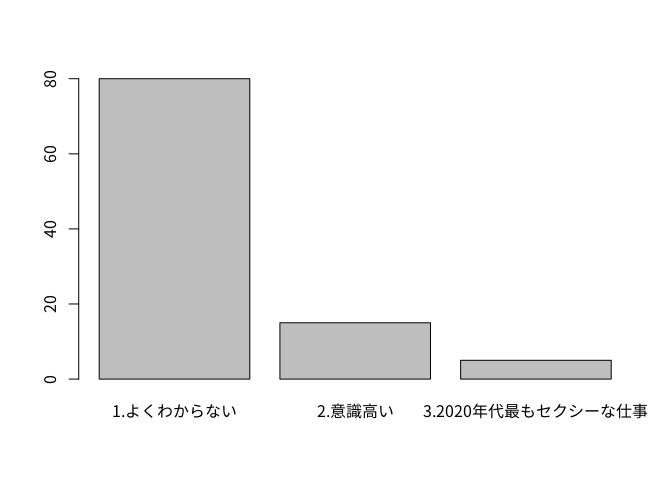
\includegraphics{Presentation_files/figure-beamer/unnamed-chunk-1-1.pdf}

\end{frame}

\section{きぬいともよくわかんない}

\begin{frame}{「意識高い」マーケティングあるある}

\begin{itemize}
\tightlist
\item
  「ドリルを買う人は、ドリルがほしいんじゃなくて、穴がほしいんだよ」
\end{itemize}

\begin{itemize}
\tightlist
\item
  新人だったころのきぬいと「そう\ldots{}\ldots{}(無関心)」
\end{itemize}

\end{frame}

\begin{frame}{「マーケティング」のよくわからなさ}

\begin{itemize}
\tightlist
\item
  どうなったら「うまくいった」と言えるのかがよくわからない

  \begin{itemize}
  \tightlist
  \item
    測定指標(KDIだのKPIだの)がうまく定義されていない
  \item
    あるいは大きく定義変更がなされる
  \end{itemize}
\item
  データがどう使えるのか問題

  \begin{itemize}
  \tightlist
  \item
    大体の日本企業はデータはある

    \begin{itemize}
    \tightlist
    \item
      でも扱えない
    \end{itemize}
  \end{itemize}
\end{itemize}

\end{frame}

\begin{frame}{界隈の動向}

\begin{itemize}
\tightlist
\item
  KKD(経験・勘・度胸)への信頼が篤い

  \begin{itemize}
  \tightlist
  \item
    実際その道のベテランのKKは馬鹿にはできない(くやしい)
  \item
    実際Dなしに決定はできない(それはそう)
  \item
    データ分析の価値もKKDに合うかどうかで決まるところもある
  \end{itemize}
\end{itemize}

\end{frame}

\begin{frame}{(画像)}

\end{frame}

\end{document}
